\documentclass[thesis.tex]{subfiles}

\begin{document}


\chapter{The digestive system}  \label{the_digestive_system}
%-----------------------------------------------------------
%what to look for when analyzing videos from the digestive system

To detect irregularities in the digestive system (Figure \ref{fig:digestive_system}) is a difficult and time-consuming task. To classify irregularities correctly and precisely require expert knowledge. Fortunately we have access to data which already has been labeled by trained professionals that we will use in this project.

The most common way of screening patients is with a endoscope. When this tool is used by a professional some of the irregularities that can be spotted are; \textit{Colon polyp}, \textit{Colorectal Cancer}, \textit{Ulcerative Colitis}, \textit{Crohn's Disease}, \textit{Familial adenomatous polypsis}, \textit{Diverticulosis} and \textit{Diverticula Bleeding}. 

These diseases have varying patterns and while some can be easy to split apart, some are more similar in pattern. While for an untrained eye it can be easy to spot that something is wrong it is very difficult to describe with words what that might be or even harder to write a program to detect the correct characteristic features of the disease. This is why we rely on having good amount of labeled data for this project to work. For increased accuracy we may have to look closer at a couple of diseases. Preferably two irregularities that both have different characteristics and lots of labeled training data.

\begin{figure}[h] % digestive-system
  \begin{center}
    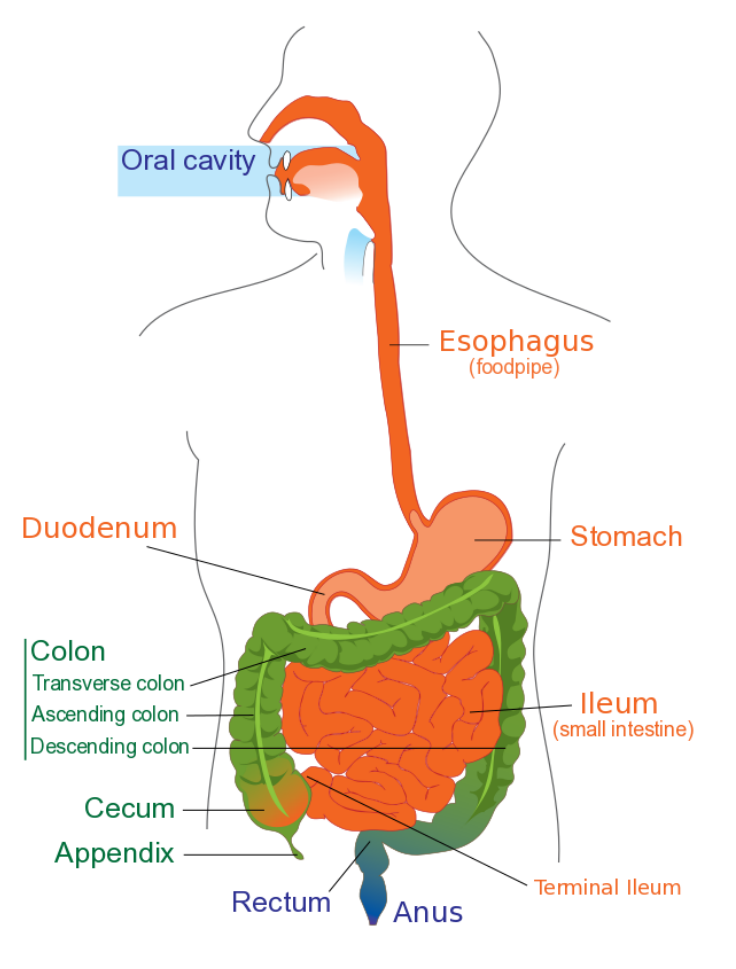
\includegraphics[width=0.5\textwidth]{digestive-system}
    \caption[Image]{An overview of the terms used to describe the digestive system\footnotemark.}
    \label{fig:digestive_system}
  \end{center}
\end{figure}

\footnotetext{
\text{By Mariana Ruiz, edited by Joaquim Gaspar. Released into public domain by author.} \newline
\url{https://en.wikipedia.org/wiki/File:Digestive_system_diagram_edit.svg}
}



\end{document}